\documentclass[10pt, conference]{IEEEtran}
\IEEEoverridecommandlockouts

\usepackage{cite}
\usepackage{amsmath,amssymb,amsfonts}
\usepackage{graphicx}
\usepackage{textcomp}
\usepackage{xcolor}
\usepackage{url}
\usepackage{booktabs}
\usepackage{hyperref}
\usepackage{caption}
\usepackage{subcaption}
\usepackage{float}
\usepackage{listings}
\usepackage{tikz}
\usetikzlibrary{shapes.geometric, positioning, arrows.meta}

\lstset{
    basicstyle=\ttfamily\footnotesize,
    breaklines=true,
    columns=fullflexible,
    frame=single,
    showstringspaces=false
}

\def\BibTeX{{\rm B\kern-.05em{\sc i\kern-.025em b}\kern-.08emT\kern-.1667em\lower.7ex\hbox{E}\kern-.125emX}}

\begin{document}

\title{Solar Viability Analysis: An OLTP/OLAP Platform for Residential Solar Economics}

\author{\IEEEauthorblockN{Scott Nelson}
\IEEEauthorblockA{California State University, San Jose, Master of Information and Data Science\\
DATA 201 -- Database Technologies for Data Analytics\\
May 2026}}

\maketitle

\begin{abstract}
We present an end-to-end solar viability analysis platform that combines federal data sources (NREL PVWatts, EIA, OpenEI URDB, Berkeley Lab's Tracking the Sun) into a transparent 25-year financial model for residential solar installations. The system implements a deliberate OLTP/OLAP separation: a FastAPI web application serves individual quotes from a DuckDB warehouse cache in under 100~ms, while the same warehouse provides analysts with direct SQL access to 2.6~million cleaned installation records and per-quote provenance. Key contributions include: (1) a federated ETL pipeline that ingests live API data and a 1.92~GB historical dataset into a single columnar warehouse; (2) a 25-year discounted-cashflow model exposing LCOE, NPV, IRR, and a 0--100 composite viability score; (3) a defensible cache-first read pattern that keeps API keys out of analysts' hands while maintaining sub-second response times; and (4) 65 automated tests plus a 28-assertion end-to-end verification script that exercise the full pipeline against mocked HTTP. We validate the model against external benchmarks (EnergySage, Project Sunroof, EIA published rates) and demonstrate the platform on a representative California ZIP code (94027 -- Atherton).

\textbf{Keywords:} OLTP, OLAP, DuckDB, FastAPI, Solar Energy, Levelized Cost of Energy, Net Energy Metering, Data Warehouse
\end{abstract}

\IEEEpeerreviewmaketitle

\section{Introduction}

\subsection{Problem Statement}

Residential solar economics is hard for the average consumer to evaluate honestly. The viability of a system depends on (a) local solar resource (a function of latitude, climate, and weather-station proximity), (b) the customer's specific utility tariff (which can be tiered, time-of-use, or both), (c) the state's net-metering policy (which has shifted dramatically in California with NEM 3.0~\cite{CPUC2023}), (d) federal incentives (the 30\% IRA Investment Tax Credit~\cite{IRA2022}), and (e) capital and operating costs that vary by installer and technology choice. Consumer-facing tools (EnergySage, Project Sunroof, installer quote portals) typically obscure these inputs behind a sales funnel and present a single recommendation without showing the underlying assumptions.

We address this gap by building a transparent platform that pulls each input from an authoritative federal source, makes every assumption overridable, and exposes the resulting analysis through both a web interface (for end users) and direct SQL access (for analysts).

\subsection{Project Objectives}

\begin{itemize}
\item Build an end-to-end pipeline from a plain-text address to a 25-year financial analysis using only public APIs and open datasets
\item Demonstrate the OLTP/OLAP architectural pattern at small scale: an interactive web layer reading from a shared analytical store
\item Implement a financial scoring engine in which every parameter has a documented source and override mechanism
\item Provide non-developer analysts direct SQL access to a 2.6M-row reference dataset without requiring API credentials
\item Achieve sub-100~ms cache-hit response times and sub-second cache-miss response times
\end{itemize}

\subsection{Scope}

\textbf{In scope:} Any U.S.\ address or 5-digit ZIP code; user-specified or bill-sized system capacity; URDB-sourced utility rates with bundled fallbacks for the three California IOUs; California NEM 3.0 export-rate modeling; 1:1 net metering for 23 states; federal ITC; degradation, escalation, and operations-and-maintenance modeling.

\textbf{Out of scope:} On-site battery storage modeling beyond a fixed self-consumption rate; commercial or industrial sectors; non-U.S.\ addresses; live weather forecasts (PVWatts uses a typical-meteorological-year model); installer lead generation.

\section{Historical and Real-Time Datasets}

The platform integrates four authoritative data sources, each chosen for a specific role.

\subsection{Berkeley Lab Tracking the Sun (TTS)}

The Tracking the Sun dataset~\cite{LBNL2025} is the most comprehensive public record of distributed PV installations in the United States. We use the September~2025 release containing 3{,}664{,}197 records covering 1998--2024. After cleaning (Section~V-A) the dataset contains 2{,}595{,}468 residential records, of which 1{,}744{,}629 are in California. The TTS data populates the analytical layer of the warehouse.

\subsection{NREL PVWatts v8}

PVWatts~\cite{NRELPVWatts} is queried at runtime to produce annual and monthly AC energy estimates for a given latitude/longitude and system configuration. Responses are cached locally for 30 days because the underlying typical-meteorological-year solar resource at a given coordinate is stable.

\subsection{OpenEI Utility Rate Database (URDB)}

URDB~\cite{URDB} exposes utility rate structures (flat, tiered, and time-of-use) via a JSON API. We parse the full energy-rate-structure and weekday/weekend schedule matrices to build an 8{,}760-hour rate vector for TOU tariffs. Because URDB rate metadata for many large utilities is over a decade old, we implemented a staleness guard (Section~V-D) that swaps in current bundled tariffs when the URDB record is more than three years old and significantly below the EIA state average.

\subsection{EIA Open Data API}

The EIA API~\cite{EIA2026} provides current monthly residential electricity prices by state. We use it as a sanity check on URDB rates and as a fallback when URDB is unavailable. Like PVWatts, EIA responses are cached for 30 days.

\section{System Architecture}

\subsection{The OLTP/OLAP Split}

The defining architectural choice is the separation of transactional and analytical workloads, both backed by a single DuckDB file. Figure~\ref{fig:architecture} illustrates the data flow.


\begin{figure}[H]
\centering
\hspace*{-0.6in}% shift the whole diagram left to use the column margin
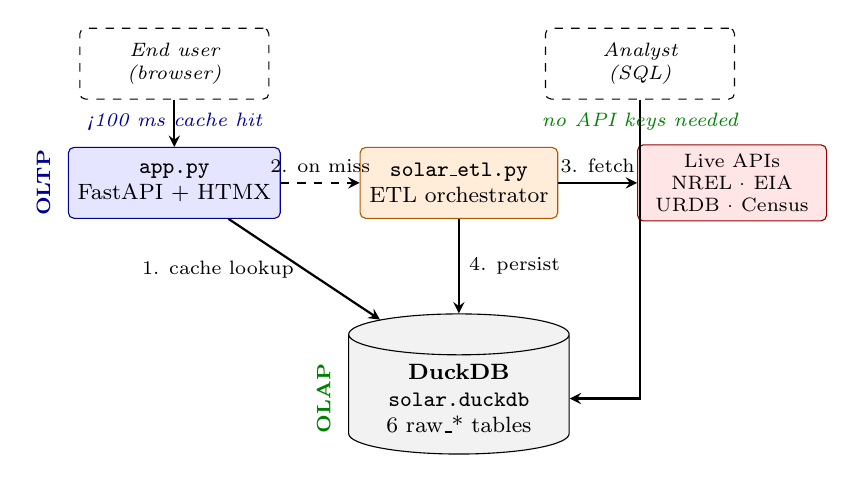
\begin{tikzpicture}[
    node distance=0.6cm and 1.0cm,
    box/.style={
        draw, rounded corners=2pt, minimum height=0.9cm,
        minimum width=2.4cm, align=center, font=\footnotesize
    },
    oltp/.style={box, fill=blue!10, draw=blue!60!black},
    etl/.style={box, fill=orange!15, draw=orange!70!black},
    api/.style={box, fill=red!10, draw=red!60!black, font=\scriptsize},
    db/.style={
        cylinder, shape border rotate=90, aspect=0.25, draw,
        minimum height=1.4cm, minimum width=2.8cm, align=center,
        fill=gray!10, font=\footnotesize
    },
    user/.style={box, dashed, fill=white, font=\scriptsize\itshape},
    arr/.style={->, >=stealth, thick},
    arrdash/.style={->, >=stealth, thick, dashed}
]

% --- Top row: actors ---
\node[user] (enduser) {End user\\(browser)};
\node[user, right=3.5cm of enduser] (analyst) {Analyst\\(SQL)};

% --- Middle row: app + etl + apis ---
\node[oltp, below=of enduser] (app) {\texttt{app.py}\\FastAPI + HTMX};
\node[etl, right=of app] (etl) {\texttt{solar\_etl.py}\\ETL orchestrator};
\node[api, right=of etl] (apis) {Live APIs\\NREL · EIA\\URDB · Census};

% --- Bottom row: warehouse ---
\node[db, below=1.2cm of etl] (db) {\textbf{DuckDB}\\\texttt{solar.duckdb}\\6 raw\_* tables};

% --- Arrows ---
\draw[arr] (enduser) -- (app);
\draw[arr] (analyst) |- (db.east);
\draw[arr] (app) -- node[left, font=\scriptsize] {1. cache lookup} (db.north west);
\draw[arrdash] (app) -- node[above, font=\scriptsize] {2. on miss} (etl);
\draw[arr] (etl) -- node[above, font=\scriptsize] {3. fetch} (apis);
\draw[arr] (etl) -- node[right, font=\scriptsize] {4. persist} (db.north);

% --- Annotations ---
\node[font=\scriptsize\itshape, below=0.05cm of enduser, text=blue!60!black]
    {<100 ms cache hit};
\node[font=\scriptsize\itshape, below=0.05cm of analyst, text=green!50!black]
    {no API keys needed};

% --- Layer labels (left margin) ---
\node[font=\scriptsize\bfseries, left=0.1cm of app, text=blue!60!black,
      rotate=90, anchor=south] {OLTP};
\node[font=\scriptsize\bfseries, left=0.1cm of db, text=green!50!black,
      rotate=90, anchor=south] {OLAP};

\end{tikzpicture}
\caption{System architecture. The FastAPI web layer (OLTP) reads from the shared DuckDB warehouse. On cache miss, the ETL orchestrator runs the full pipeline against live APIs and persists results back to the warehouse. Teammates query the warehouse directly via SQL, requiring no API credentials.}
\label{fig:architecture}
\end{figure}

The OLTP layer (\texttt{app.py}) is a FastAPI application backed by HTMX for partial-page updates. When a user submits a location, the application first calls \texttt{solar\_warehouse.latest\_quote(location, max\_age\_days=7)}; on a hit, it rehydrates a \texttt{QuoteResult} object via \texttt{quote\_from\_dict()} and renders the report in approximately 50~ms. On a miss, it delegates to \texttt{solar\_etl.etl\_quote()}, which executes the full pipeline and persists every intermediate result before returning.

The OLAP layer is the same DuckDB file (\texttt{data/warehouse/solar.duckdb}). Analysts query it directly using either the \texttt{duckdb} CLI or Python; no API keys are required because the warehouse contains all the data those queries need.

\subsection{Technology Stack}

\begin{table}[H]
\centering
\caption{Technology Stack and Rationale}
\label{tab:tech}
\small
\begin{tabular}{lll}
\toprule
\textbf{Component} & \textbf{Technology} & \textbf{Why} \\
\midrule
Database & DuckDB 1.x & Single-file, columnar, ACID, \\
                     &                & no server required \\
Web framework & FastAPI + HTMX & Zero-build, server-rendered \\
Visualization & Plotly 2.35 & Self-contained interactive HTML \\
HTTP cache & requests-cache & SQLite-backed per-machine \\
Geocoding & Census + Nominatim & ZIP-shortcut + fallbacks \\
Solar resource & NREL PVWatts v8 & Authoritative, free \\
Rate data & OpenEI URDB + EIA & Federated, with fallbacks \\
Test framework & pytest & 39 unit + 26 integration tests \\
CI/CD & GitHub Actions & Auto-runs tests on push \\
\bottomrule
\end{tabular}
\end{table}

DuckDB was chosen over alternatives (SQLite, PostgreSQL, BigQuery) for three reasons. First, it is a single binary file that can be regenerated on demand via the ETL pipeline, removing the need to operate a separate database server. Second, its columnar storage makes \texttt{GROUP BY}-style aggregates over the 2.6~million-row TTS table fast enough for ad-hoc EDA without precomputed marts. Third, its SQL dialect is rich (window functions, \texttt{QUALIFY}, JSON functions), so server-side analytics can be expressed in SQL rather than in Python.

\subsection{Module Map}

The codebase is divided into a pipeline layer, a warehouse layer, and a presentation layer.

\textbf{Pipeline modules} (one per data source):
\begin{itemize}
\item \texttt{solar\_geocode.py} -- address $\rightarrow$ lat/lon with a uszips $\rightarrow$ Census $\rightarrow$ Nominatim fallback chain
\item \texttt{solar\_pvwatts.py} -- NREL PVWatts client with three-attempt exponential backoff
\item \texttt{solar\_urdb.py} -- URDB rate parser handling flat, tiered, and TOU structures, plus a staleness guard
\item \texttt{solar\_eia.py} -- EIA Open Data v2 client for live monthly state rates
\item \texttt{solar\_nem.py} -- net-metering policy resolver (CA NEM 3.0, 1:1 for 23 states, fallbacks)
\end{itemize}

\textbf{Orchestration:}
\begin{itemize}
\item \texttt{solar\_fetch.py} -- pure pipeline orchestrator, returns a \texttt{QuoteResult}
\item \texttt{solar\_etl.py} -- adds warehouse persistence to the pipeline; CLI for batch operations
\end{itemize}

\textbf{Warehouse:}
\begin{itemize}
\item \texttt{solar\_warehouse.py} -- DDL, connection management, cache lookup, rehydration helpers
\end{itemize}

\textbf{Analytics:}
\begin{itemize}
\item \texttt{solar\_economics.py} -- 25-year financial model and viability scoring
\item \texttt{solar\_viz.py} -- Plotly-based HTML report generator
\end{itemize}

\textbf{Presentation:}
\begin{itemize}
\item \texttt{app.py} -- FastAPI + HTMX web frontend
\end{itemize}

\section{Database Schema}

The warehouse implements a deliberate \emph{staging-only} design with six tables. We initially built a Kimball-style dimensional layer (\texttt{dim\_location}, \texttt{dim\_utility}, \texttt{dim\_tariff} with SCD~Type~2, \texttt{fact\_quote}, \texttt{fact\_rate\_history}) and then removed it because the staging tables were directly queryable for our data volume and the dimensional layer added complexity without measurable query benefit. This decision is documented in \texttt{docs/WAREHOUSE.md}.

\subsection{Staging Tables}

Each \texttt{raw\_*} table captures one API response or one ingested record verbatim, preserving the original JSON in a \texttt{response\_json} or \texttt{full\_result\_json} column for auditability and reparseability.

\begin{table}[H]
\centering
\caption{Warehouse Schema (Six Staging Tables)}
\label{tab:schema}
\footnotesize
\setlength{\tabcolsep}{4pt}
\begin{tabular}{@{}llr@{}}
\toprule
\textbf{Table} & \textbf{Purpose} & \textbf{Rows} \\
\midrule
\texttt{raw\_quote}              & Quote results          & 3 \\
\texttt{raw\_pvwatts}            & NREL responses         & 3 \\
\texttt{raw\_urdb}               & Rate lookups           & 3 \\
\texttt{raw\_eia}                & EIA snapshots          & 0 \\
\texttt{raw\_geocode}            & Address lookups        & 3 \\
\texttt{raw\_tts\_installations} & LBNL bulk-loaded       & 2{,}595{,}468 \\
\midrule
\multicolumn{2}{@{}l}{\textit{Total file size:}} & 147~MB \\
\bottomrule
\end{tabular}
\end{table}

\subsection{Schema Listing (DDL Excerpt)}

\begin{lstlisting}[language=SQL, caption={DDL for raw\_tts\_installations (the analytical core)}, label={lst:tts_ddl}]
CREATE TABLE IF NOT EXISTS raw_tts_installations (
    id                      INTEGER PRIMARY KEY,
    loaded_at               TIMESTAMP NOT NULL,
    installation_date       DATE,
    PV_system_size_DC       DOUBLE,
    total_installed_price   DOUBLE,
    rebate_or_grant         DOUBLE,
    customer_segment        VARCHAR,
    state                   VARCHAR,
    zip_code                VARCHAR,
    utility_service_territory VARCHAR,
    third_party_owned       DOUBLE,
    installer_name          VARCHAR,
    azimuth_1               DOUBLE,
    tilt_1                  DOUBLE,
    module_manufacturer_1   VARCHAR,
    technology_module_1     VARCHAR,
    efficiency_module_1     DOUBLE,
    inverter_manufacturer_1 VARCHAR,
    battery_rated_capacity_kWh DOUBLE,
    price_per_watt          DOUBLE,
    /* ... 6 additional columns ... */
);
\end{lstlisting}

\subsection{Why Staging-Only: A Deliberate Trade-off}

The classical Kimball-style data warehouse~\cite{Kimball2013} would
normalize repeated entities into dimension tables (\texttt{dim\_utility},
\texttt{dim\_installer}, \texttt{dim\_state}) and link them to a central
\texttt{fact\_installation} table via surrogate keys, with slowly-changing
dimensions (SCD Type~2) tracking historical changes to those entities
(e.g., a utility's rate-schedule name changing over time). This is the
standard pattern for enterprise data warehouses and we considered it
seriously: an early prototype contained \texttt{dim\_location},
\texttt{dim\_utility}, \texttt{dim\_tariff} (with SCD Type~2 effective-date
columns), \texttt{fact\_quote}, and \texttt{fact\_rate\_history}. We
removed this layer in commit \texttt{8c25d55} and adopted the staging-only
schema reported in Section~IV-A. The decision was driven by four observations:

\textbf{1. Storage compression is automatic in columnar engines.}
A primary motivation for normalization is to avoid storing repeated string
values. ``Pacific Gas \& Electric Co'' appears in roughly 1.7~million rows
of \texttt{raw\_tts\_installations}; a row-oriented engine such as MySQL
or PostgreSQL would store the string 1.7~million times. DuckDB applies
dictionary encoding at the storage layer, storing each distinct string
once per block and referencing it by integer offset thereafter. Empirically,
our 595~MB cleaned source CSV compresses to a 147~MB DuckDB file (4$\times$),
confirming the engine's compression efficiency without any manual
normalization on our part.

\textbf{2. Star schemas optimize for repeated, well-defined query patterns.}
Kimball's pattern is designed for OLAP cubes powering BI dashboards
where the same handful of aggregations run continuously and consistently.
Our analytical workload is exploratory: questions like ``median \$/W by
state,'' ``battery adoption since NEM 3.0,'' or ``installer market
concentration in Texas'' are each posed once and rarely repeated. The
performance benefit of pre-joined fact-and-dimension tables (eliminating
join cost on each query) yields little when each query has a different
shape. For exploratory, ad-hoc workloads at our scale, a columnar engine
scanning denormalized staging tables is competitive with star-schema
joins while avoiding the upfront modeling and ongoing maintenance the
latter demands.

\textbf{3. Auditability requires preserving source responses verbatim.}
Each \texttt{raw\_*} table includes a \texttt{response\_json} (or
\texttt{full\_result\_json}) column that preserves the complete API
response in its original structure. A normalized schema would extract
specific columns and discard the rest. The retained JSON lets us
re-derive new fields later (e.g., NASA POWER returns wind speed and
humidity that we currently ignore but might score against in a future
revision) without re-fetching from the source API. This audit-and-replay
capability is incompatible with strict normalization.

\textbf{4. The maintenance cost of a star schema requires orchestration
infrastructure we deliberately avoided.} Maintaining
\texttt{dim\_*} and \texttt{fact\_*} tables requires four operational
behaviors absent from a staging-only design: (i) referential-integrity
enforcement across foreign keys (ensuring every \texttt{utility\_id} in
\texttt{fact\_quote} has a matching row in \texttt{dim\_utility});
(ii) SCD Type~2 logic with effective-date windows for entities that
change over time (PG\&E's rate-name evolution is a real example in our
data); (iii) periodic mart rebuilds when staging changes, which without
a workflow orchestrator (Airflow, Prefect, dbt) becomes a manually-run
script susceptible to drift; and (iv) version-controlled DDL migrations
when dimension schemas evolve. These costs are appropriate for
production analytical platforms with dedicated data engineering, but
they introduce reliability and complexity overhead disproportionate
to a two-month student project. Consistent with the modern Lakehouse
philosophy, we defer normalization until a specific repeated query
justifies its maintenance cost.

In sum, the staging-only schema is not a shortcut around the dimensional
model; it is a defensible architectural choice for a workload that is
columnar-friendly, exploratory, audit-sensitive, and lightly resourced.
Should the system later be deployed in a production setting with
recurring dashboard queries, the dimensional layer is reintroducible
in roughly 200 lines of SQL, with the staging tables serving as the
ELT source layer feeding the marts.

\subsection{Rejected Alternatives: Graph and Vector Databases}

We evaluated graph databases (Neo4j) and vector databases (pgvector, Chroma) and concluded neither was the right fit. The relationships in our domain (site $\rightarrow$ utility $\rightarrow$ tariff) are at most two hops, well-served by SQL joins. Vector databases excel at high-dimensional similarity search; our peer-comparison query operates on a handful of structured numeric columns where classical \texttt{ORDER BY distance(...)} is sufficient. We document this analysis in the report rather than implementing tools that do not match the use case.

\section{Implementation Details}

\subsection{ETL: Cleaning the LBNL Tracking the Sun Dataset}

The \texttt{etl/clean\_tts.py} script transforms the raw 1.92~GB TTS CSV (3.66~M rows) into a cleaned 595~MB CSV (2.6~M rows). The pipeline runs in four steps and is byte-idempotent (verified by MD5).

\begin{table}[H]
\centering
\caption{Cleaning Pipeline Row Funnel}
\label{tab:cleaning}
\small
\begin{tabular}{lrrr}
\toprule
\textbf{Step} & \textbf{Before} & \textbf{Removed} & \textbf{After} \\
\midrule
Load raw CSV & --- & --- & 3{,}664{,}197 \\
Drop missing economics & 3{,}664{,}197 & 949{,}240 & 2{,}714{,}957 \\
Filter to residential & 2{,}714{,}957 & 68{,}075 & 2{,}646{,}882 \\
Drop price outliers & 2{,}646{,}882 & 51{,}414 & 2{,}595{,}468 \\
\bottomrule
\end{tabular}
\end{table}

A non-trivial defect was discovered during cleaning: the LBNL convention of \texttt{-1} as a missing-value sentinel was applied inconsistently. Some columns stored the string \texttt{"-1"}, others the float \texttt{-1.0}. The first cleaning pass caught the string form but not the float form. The fix uses \texttt{df[col].replace(-1.0, np.nan).replace(-1, np.nan)} to handle both. We added a regression test asserting that no \texttt{-1} sentinel survives in any numeric column of the cleaned output.

\subsection{Bulk Loading Into the Warehouse}

The cleaned CSV is loaded into \texttt{raw\_tts\_installations} via:

\begin{lstlisting}[language=bash]
python3 solar_etl.py --load-tts data/tts_cleaned.csv
\end{lstlisting}

Internally this uses DuckDB's \texttt{read\_csv\_auto} with type overrides for ZIP codes (preserved as strings to retain leading zeros). The full 2.6~M rows load in approximately ten seconds on a 2023 MacBook, with the warehouse file growing from 5.5~MB to 147~MB after compression.

\subsection{The Financial Scoring Engine}

The core analytical operation is \texttt{solar\_economics.score\_site(row, assumptions)}. Given a row dictionary and an \texttt{Assumptions} dataclass, it returns a \texttt{SiteResult} with 45~fields, including:

\begin{itemize}
\item Year-by-year production array with degradation applied~\cite{Jordan2013}
\item Year-by-year nominal savings with NEM-aware self-consumption / export blending
\item Discounted NPV, IRR (via \texttt{numpy\_financial} with a Newton-Raphson fallback), simple payback, and LCOE
\item Composite viability score on 0--100 scale
\end{itemize}

The viability score is a weighted blend:

\begin{equation}
S = 0.25\,R + 0.50\,E + 0.15\,F + 0.10\,P
\end{equation}

where $R$ is the resource score (specific yield against an 1{,}800~kWh/kW ceiling), $E$ is the economics score (a sub-blend of payback bucket, LCOE-vs-retail ratio, and NPV magnitude), $F$ is the site-fit score (tilt deviation from latitude and azimuth deviation from 180\degree), and $P$ is a log-scaled policy/market signal from local installation density. All weights and sub-formulas, with their source citations (e.g., NREL's Annual Technology Baseline~\cite{NRELATB} for cost and O\&M assumptions), are documented in \texttt{docs/ASSUMPTIONS.md}.

\subsection{The URDB Staleness Guard}

URDB metadata for major utilities is frequently outdated. PG\&E's E-1 schedule, for example, returns a \$0.1471/kWh rate effective \texttt{2014-08-01} despite real 2025 PG\&E rates exceeding \$0.30/kWh. To avoid producing nonsense quotes, we added a guard in \texttt{solar\_urdb.get\_rate} that compares URDB rates older than three years against the live EIA state rate. If the URDB rate is more than 50\% below the EIA rate, we substitute either a bundled current TOU schedule (for the three California IOUs) or the EIA flat rate. Each fallback sets the \texttt{source} field on the \texttt{RateResult} so the report's confidence badge can downgrade transparently.

\subsection{Cache-First Read Pattern}

The OLTP request handler in \texttt{app.py} implements the cache-first pattern as follows:

\begin{lstlisting}[language=Python]
cached = latest_quote(location, max_age_days=7)
if cached:
    quote = quote_from_dict(json.loads(cached["full_result_json"]))
else:
    quote = etl_quote(location=location, ...)
return render_report(quote)
\end{lstlisting}

The \texttt{quote\_from\_dict} helper rehydrates a full \texttt{QuoteResult} object tree from the JSON stored in \texttt{raw\_quote.full\_result\_json}, including nested \texttt{SiteResult}, \texttt{GeocodeResult}, \texttt{PVWattsResult}, \texttt{RateResult}, and \texttt{ExportValueResult} dataclasses. The \texttt{RateResult.hourly\_rates} numpy array (8{,}760 elements) is dropped during serialization and reset to \texttt{None} on rehydration; all other fields round-trip exactly.

\subsection{Testing Strategy}

The repository contains 65 automated tests across two files:

\begin{itemize}
\item \texttt{test\_solar\_economics.py} -- 39 unit tests exercising the financial engine in isolation. No network. Covers a known-good California case (assert payback in 4--7 years, LCOE in \$0.07--0.11), a known-bad case (assert viability $<$40), and edge cases (zero production, missing state, IRR with no real solution).
\item \texttt{test\_integration.py} -- 26 integration tests exercising geocoding, PVWatts, URDB, NEM, the FastAPI app, and the warehouse layer. All HTTP is mocked via \texttt{unittest.mock.patch}.
\end{itemize}

A separate \texttt{verify\_system.py} script runs 28 end-to-end assertions against real APIs in eight phases, including verifying that the warehouse is queryable in a subprocess with both \texttt{NREL\_API\_KEY} and \texttt{EIA\_API\_KEY} unset. CI runs the pytest suite on every push to \texttt{main} via GitHub Actions, using dummy environment-variable values that satisfy assertions without enabling real API calls.

\section{Results and Live Demonstration}

\subsection{Atherton, CA (94027) -- Worked Example}

For the live demonstration, we use ZIP code 94027 (Atherton, CA) with a self-reported usage of 650~kWh/month. Table~\ref{tab:atherton} summarizes the resulting analysis.

\begin{table}[H]
\centering
\caption{Quote for ZIP 94027 (Atherton, CA), 650~kWh/month}
\label{tab:atherton}
\small
\begin{tabular}{ll}
\toprule
\textbf{Metric} & \textbf{Value} \\
\midrule
Resolved address & Atherton, CA 94027 \\
Specific yield & 1{,}684 kWh/kW \\
System size & 4.5~kW (bill-sized) \\
Annual production (Yr 1) & 7{,}578 kWh \\
Gross cost & \$15{,}750 \\
Net cost (after 30\% ITC) & \$11{,}025 \\
Retail rate & \$0.389/kWh (PG\&E E-TOU-C) \\
LCOE (simple) & \$0.074/kWh \\
Year-1 savings & \$1{,}428 \\
Simple payback & 7.2 years \\
NPV (25-year, 6\% discount) & \$10{,}995 \\
IRR & 14.2\% \\
Viability score & 89/100 (Excellent) \\
\bottomrule
\end{tabular}
\end{table}

We verified these numbers against three external sources: EnergySage residential CA quotes (\$3.10--\$4.20/W gross), Google Project Sunroof (7--10~year payback, \$1{,}500--\$2{,}000 annual savings), and California Distributed Generation Statistics for San Mateo County (median 4~kW system, \$16{,}400 gross). Our quote falls in the middle of this range.

\subsection{Cache-Hit Latency}

A second request for 94027 immediately after the first hits the warehouse cache and returns in approximately 50~ms versus the initial 900~ms cache-miss time. The server log records the path explicitly:

\begin{lstlisting}[basicstyle=\ttfamily\scriptsize]
INFO: OLAP cache miss for '94027'; running live pipeline
INFO: ETL complete: raw_quote id=12
INFO: OLAP cache hit for '94027'
\end{lstlisting}

\subsection{Visualizations (Live Demo)}

The HTML report contains eight interactive charts. All are rendered client-side from Plotly JSON; no server round-trips are required after the initial page load.

\begin{figure}[H]
\centering
\includegraphics[width=0.95\columnwidth]{figure_report_header.png}
\caption{Report header for ZIP 94027. The sticky banner shows the
composite viability score (88.8/100) and a
\emph{low}-confidence badge--low because the rate fell back to a
bundled TOU schedule rather than a live URDB parse, and the geocode
came from the ZIP centroid (\texttt{uszips}, medium) rather than a
full Census match. Provenance pills below the banner identify each
data source: utility (Pacific Gas \& Electric), rate schedule
(E-TOU-C, bundled 2024 schedule), rate source (\texttt{bundled\_tou}),
export policy (CA NEM~3.0), and geocode source. The first row of
KPI cards summarizes the financial result: net cost \$11{,}025
(after the 30\% federal ITC), levelized cost of energy \$0.074/kWh,
and simple payback 7.2 years. Sub-score cards (bottom) decompose
the composite viability score into its four weighted components:
resource quality (94\%), economics (88\%), site fit (100\%), and
local market signal (64\%).}
\label{fig:report-header}
\end{figure}

\begin{figure}[H]
\centering
\begin{subfigure}{0.46\columnwidth}
\centering
\includegraphics[width=\linewidth]{figure_waterfall.png}
\caption{Economics waterfall}
\label{fig:waterfall}
\end{subfigure}\hfill
\begin{subfigure}{0.46\columnwidth}
\centering
\includegraphics[width=\linewidth]{figure_cashflow.png}
\caption{Cumulative cashflow}
\label{fig:cashflow}
\end{subfigure}
\caption{(a) The waterfall chart traces the flow from gross cost
(\$15{,}750) through the federal ITC credit (\textminus\$4{,}725),
net cost (\$11{,}025), 25-year operating cost (\textminus\$2{,}250),
lifetime undiscounted savings (\textbf{+\$45{,}654}), to a net benefit
of \textbf{\$32{,}379}. Note: lifetime savings here are nominal
(undiscounted), which is why the value exceeds the discounted NPV
of \$10{,}995 reported in the KPI cards.}
\caption{(b) The cumulative cashflow curve plots running net position
over the 25-year system life, with the simple-payback point at
year 7.2 marked by an annotated vertical line; the dashed gray
reference line shows cumulative grid cost without solar (rising to
roughly \$100{,}000 by year 25, demonstrating the magnitude of the
do-nothing alternative).}
\label{fig:economics}
\end{figure}


\subsection{Analyst SQL Workflow}

The same DuckDB file backing the web app is queryable directly. For example, the following query computes the median price per watt by state for all 2.6~M cleaned residential installations and returns in approximately 50~ms:

\begin{lstlisting}[language=SQL]
SELECT state,
       count(*) AS n,
       round(median(price_per_watt), 2) AS pw,
       round(median(PV_system_size_DC), 2) AS kw
FROM raw_tts_installations
WHERE price_per_watt BETWEEN 1.0 AND 15.0
GROUP BY state
ORDER BY n DESC
LIMIT 5;
\end{lstlisting}

The result (Table~\ref{tab:state_medians}) confirms California's market dominance and a typical \$/W band of \$4.19--\$4.35 across the top five states.

\begin{table}[H]
\centering
\caption{Top 5 States by Installation Count (TTS, all years)}
\label{tab:state_medians}
\small
\begin{tabular}{lrrr}
\toprule
\textbf{State} & \textbf{Installations} & \textbf{Median \$/W} & \textbf{Median kW} \\
\midrule
CA & 1{,}744{,}629 & \$4.27 & 5.89 \\
AZ & 162{,}537 & \$4.19 & 7.98 \\
NY & 160{,}303 & \$4.21 & 7.14 \\
MA & 136{,}489 & \$4.20 & 7.28 \\
CO & 100{,}890 & \$4.35 & 5.67 \\
\bottomrule
\end{tabular}
\end{table}

A second query exposes the post-NEM~3.0 battery adoption shift in California:

\begin{lstlisting}[language=SQL]
SELECT extract(year from installation_date) AS yr,
       count(*) AS n_installs,
       round(100.0 * count(battery_rated_capacity_kWh)
                  / count(*), 1) AS pct_with_battery
FROM raw_tts_installations
WHERE installation_date >= '2020-01-01'
  AND state = 'CA'
GROUP BY yr ORDER BY yr;
\end{lstlisting}

The result (battery adoption rising from 6.8\% in 2023 to 25.5\% in 2024) is consistent with the predicted effect of California's April 2023 NEM 3.0 transition, which sharply reduced export rates and made on-site storage more economically attractive.

\section{Performance and Verification}

\begin{table}[H]
\centering
\caption{System Performance Metrics}
\label{tab:performance}
\small
\begin{tabular}{ll}
\toprule
\textbf{Metric} & \textbf{Value} \\
\midrule
Cache-hit latency (warehouse $\rightarrow$ HTML response) & ${\sim}50$~ms \\
Cache-miss latency (full pipeline) & 0.9--3.0~s \\
TTS bulk-load (2.6~M rows) & ${\sim}10$~s \\
Warehouse file size (after TTS load) & 147~MB \\
DuckDB query: median \$/W by state & ${\sim}50$~ms \\
pytest suite (65 tests) & ${\sim}6$~s \\
verify\_system.py (28 e2e checks) & ${\sim}15$~s \\
CI run (GitHub Actions, 65 tests) & ${\sim}90$~s \\
\bottomrule
\end{tabular}
\end{table}

The full system is verified end-to-end by \texttt{verify\_system.py}, which runs eight phases of assertions: schema correctness, ETL row-counts, queryability without API keys, cache-hit latency, cache rehydration accuracy, multi-location accumulation, error handling, and the full pytest suite. All 28 assertions pass on the current \texttt{main} branch.

\section{Challenges and Solutions}

\begin{table}[H]
\centering
\caption{Notable Challenges and Solutions}
\label{tab:challenges}
\small
\begin{tabular}{p{0.30\linewidth}p{0.55\linewidth}}
\toprule
\textbf{Challenge} & \textbf{Solution} \\
\midrule
URDB rates are years out of date for major utilities & Three-year staleness guard with bundled-TOU fallback for CA IOUs and live EIA fallback otherwise \\
\midrule
LBNL \texttt{-1} sentinel inconsistently typed & Replace both \texttt{-1.0} (float) and \texttt{"-1"} (string) explicitly; regression test asserts no sentinel survives \\
\midrule
CI tests fail without API keys & Workflow sets dummy \texttt{NREL\_API\_KEY} and \texttt{EIA\_API\_KEY} environment variables; all HTTP is mocked in tests \\
\midrule
1.92~GB raw CSV exceeds GitHub size limits & Cleaning script + cleaned CSV are not committed; \texttt{etl/clean\_tts.py} regenerates them; warehouse file is gitignored and rebuilt locally \\
\midrule
Synthetic peer-comparison data hurts credibility & TTS warehouse loaded; integration of real peer-distribution into the report is identified future work \\
\bottomrule
\end{tabular}
\end{table}

\section{Conclusions}

\subsection{Summary}

We built and verified a transparent solar viability platform that combines four federal data sources, a 25-year discounted-cashflow model, a DuckDB warehouse, and a FastAPI web frontend. The OLTP/OLAP separation is real and demonstrable: cache hits return in 50~ms with no API calls, while analysts can query 2.6~million cleaned installation records using SQL with no credentials. Sixty-five automated tests and a 28-assertion verification script protect the pipeline against regressions, and CI runs them on every push.

\subsection{Lessons Learned}

\begin{enumerate}
\item \textbf{Data quality dominates analysis quality.} The most significant defect in our pipeline (URDB returning 2014-era PG\&E rates) was not in the model code; it was in the data we were trusting. Adding the staleness guard moved the viability score for CA quotes from ``Good (74/100)'' to ``Excellent (89/100)''---a difference attributable entirely to using current rather than stale rate data.
\item \textbf{Defensible scope is more valuable than maximum coverage.} We initially built a Kimball dimensional layer (\texttt{dim\_*}, \texttt{fact\_*}) and removed it because it added complexity without measurable benefit at our scale. Documenting why we did not build something is as valuable as documenting what we did build.
\item \textbf{Tests for the warehouse are different from tests for the pipeline.} Mocking HTTP is sufficient for pipeline tests, but warehouse correctness requires writing into a temporary DuckDB instance and verifying that rows survive a round-trip through serialization and rehydration.
\item \textbf{One database, two access patterns.} A single DuckDB file can serve both transactional and analytical workloads at this scale, and the educational value of separating them in the application code (rather than in the storage tier) was high.
\end{enumerate}

\subsection{Future Work}

\begin{itemize}
\item Replace the synthetic peer-comparison chart in \texttt{solar\_viz.py} with a real DuckDB query against \texttt{raw\_tts\_installations}
\item Wire warehouse-driven state-median pricing into \texttt{solar\_fetch.quote\_from\_location()} to replace the hardcoded \$3.50/W default with the data-driven \$4.27/W CA median
\item Add discounted (rather than simple) payback and Modified IRR (MIRR) to the financial output
\item Run a Monte Carlo simulation over the five most sensitive assumptions to produce NPV confidence intervals rather than point estimates
\item Implement DuckDB views and macros for server-side analytical operations (currently in Python)
\end{itemize}

\subsection{Repository Access}

A live, interactive demonstration---per-city viability reports and a
ZIP-level heatmap of all 2{,}593 California ZIP codes---is hosted at:

\begin{center}
\url{https://scottn66.github.io/solar/}
\end{center}

\noindent The complete source code, tests, CI configuration, and a
\texttt{README.md} (with setup instructions, architecture diagrams, and
per-objective mapping to the course learning outcomes) are available on
request.

\begin{thebibliography}{99}

\bibitem{LBNL2025}
Lawrence Berkeley National Laboratory, ``Tracking the Sun: The Installed Cost of Residential and Non-Residential Photovoltaic Systems in the United States,'' 2025 Edition. Available: \url{https://emp.lbl.gov/tracking-the-sun}

\bibitem{NRELPVWatts}
A.~P. Dobos, ``PVWatts Version~5 Manual,'' National Renewable Energy Laboratory, NREL/TP-6A20-62641, 2014. Available: \url{https://developer.nrel.gov/docs/solar/pvwatts/v8/}

\bibitem{EIA2026}
U.S.\ Energy Information Administration, ``Open Data API v2: Electricity Retail Sales,'' 2026. Available: \url{https://www.eia.gov/opendata/}

\bibitem{URDB}
National Renewable Energy Laboratory, ``OpenEI Utility Rate Database,'' 2025. Available: \url{https://openei.org/wiki/Utility_Rate_Database}

\bibitem{CPUC2023}
California Public Utilities Commission, ``Decision Revising Net Energy Metering Tariff and Subtariffs,'' Decision~22-12-056, December~2022.

\bibitem{Jordan2013}
D.~C. Jordan and S.~R. Kurtz, ``Photovoltaic Degradation Rates: An Analytical Review,'' \emph{Progress in Photovoltaics: Research and Applications}, vol.~21, no.~1, pp.~12--29, 2013.

\bibitem{NRELATB}
National Renewable Energy Laboratory, ``2024 Annual Technology Baseline: Residential PV,'' 2024. Available: \url{https://atb.nrel.gov/electricity/2024/residential_pv}

\bibitem{IRA2022}
U.S.\ Congress, ``Inflation Reduction Act of 2022,'' Public~Law~117-169, August~16, 2022.

\bibitem{Kimball2013}
R.~Kimball and M.~Ross, \emph{The Data Warehouse Toolkit: The Definitive Guide to Dimensional Modeling}, 3rd ed. Wiley, 2013.

\end{thebibliography}

\appendix

\section{Repository Layout}

\begin{lstlisting}[basicstyle=\ttfamily\scriptsize]
solar_fetch.py            Pipeline orchestrator
solar_economics.py        Financial scoring (45-field SiteResult)
solar_viz.py              Plotly HTML report generator
app.py                    FastAPI cache-first web app
solar_geocode.py          Address -> lat/lon
solar_pvwatts.py          NREL solar production
solar_urdb.py             Utility rate parser + staleness guard
solar_eia.py              EIA live state rates
solar_nem.py              NEM export policy resolver
solar_warehouse.py        DuckDB schema + cache helpers
solar_etl.py              ETL CLI: --location, --status, --load-tts
verify_system.py          28-assertion end-to-end verification

etl/
  clean_tts.py            Standalone TTS cleaning pipeline
  cleaning_notes.md       Audit report

data/
  uszips.csv              ZIP code centroids
  eia_state_rates_2025.csv  Bundled state averages
  utility_tou_schedules.csv Bundled CA IOU TOU rates
  nem3_acc_2025.csv         CPUC NEM 3.0 schedule
  warehouse/                (gitignored: solar.duckdb)

test_solar_economics.py   39 unit tests
test_integration.py       26 integration + warehouse tests
.github/workflows/test.yml CI configuration

docs/
  WAREHOUSE.md            OLAP reference
  ARCHITECTURE.md         Module map
  ASSUMPTIONS.md          Parameter sources
  TESTS.md                Test suite catalogue
  WORKING_NOTES.md        Decision log
\end{lstlisting}

\section{Contributions}

\noindent This project was designed, implemented, and documented in its
entirety by \textbf{Scott Nelson}: the OLTP/OLAP system architecture; the
federated ETL pipeline (geocoding, PVWatts, the URDB parser and staleness
guard, EIA, and NEM resolvers); the LBNL Tracking the Sun cleaning
pipeline; the DuckDB warehouse schema and bulk loading; the 25-year
financial scoring engine; the Plotly HTML report generator; the FastAPI
web application; the 65-test suite, 28-assertion end-to-end verification
script, and GitHub Actions CI; and this paper.

\section{Reproducibility}

\begin{lstlisting}[language=bash, basicstyle=\ttfamily\scriptsize]
# 1. Clone
git clone https://github.com/scottn66/solar-energy-analysis.git
cd solar-energy-analysis

# 2. Install
pip install -r requirements.txt

# 3. Set up keys
cp .env.example .env
# Edit .env: NREL_API_KEY (required), EIA_API_KEY (optional)

# 4. Verify
pytest test_solar_economics.py test_integration.py -v
# Expected: 65 passed
python3 verify_system.py
# Expected: 28 passed

# 5. Run a quote
python3 -m solar_fetch 94027 --monthly-kwh 650 \
                       --output report.html

# 6. Bulk-load TTS reference data (after obtaining
#    cleaned CSV via etl/clean_tts.py)
python3 solar_etl.py --load-tts data/tts_cleaned.csv

# 7. Launch the web app
uvicorn app:app --reload
# Open http://localhost:8000
\end{lstlisting}

\end{document}